% Just The Docs Front Matter
% title: Glacial Isostatic Adjustment (GIA) Solution
% parent: Capabilities
% has_children: false
% has_toc: false

\subsection{Glacial Isostatic Adjustment (GIA) Solution} \label{sec:using-issm-capabilities-gia}

\subsubsection{Physical basis}
The ISSM/GIA model assumes that the ice sheet rests on top of the solid Earth, which is considered to be a simple two-layered incompressible continuum with upper elastic lithosphere floating on the viscoelastic (Maxwell material) mantle half-space. Coordinate transformations allow simple axisymmetric solutions for the deformation of pre-stressed solid Earth (subject to a normal surface traction of ice/ocean) to retrieve semi-analytical solutions of vertical displacement at the lithosphere surface.

\subsubsection{Vertical surface displacement}
Vertical displacement at the lithosphere surface (i.e., ice/ocean-bedrock interface), $w(r,t)$, is the most relevant field variable for GIA assessment. For brevity, hereinafter, this is referred to as the GIA solution. Semi-analytical GIA solution is given by \cite{Ivins1999}:
\begin{equation}
	w(r,t) = \int_{0}^{\infty} { k \left[ \frac{4 \mu_1^{e} \alpha}{2k\mu_1^e + \rho_1 g} \,
	\hat{Q}_0(k,t) J_1(k\alpha) \right] J_0(kr) \, \text{d}k },
\end{equation}
where:
\begin{itemize}
	\item $r$ is the radial distance from the center of the cylindrical disc load
	\item $t$ is the evaluation time
	\item $k$ is the Hankel transform variable of $r$ (or wavenumber)
	\item $\alpha$ is the radius of the cylindrical disc load
	\item $\mu_1^{e}$ is the shear modulus of elasticity of lithosphere
	\item $\rho_1$ is the lithosphere density
	\item $g$ is the vertical component of the gravity vector
	\item $J_v(kr)$ is the $v$-th order Bessel function of the first kind
	\item $\hat{Q}_0(k,t)$ accounts for the integrated influence of ice loading history
	(cf. Figure 1) at the evaluation time $t$.
	(Note that $\hat{f}_v(k)$ is the $v$-th order Hankel transform of function $f(r)$.)
\end{itemize}

\begin{figure}[h]
	\centering
	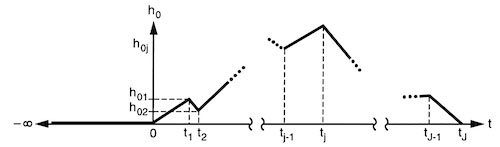
\includegraphics[width=\textwidth]{\assetsParentPath/assets/img/using-issm/capabilities/gia/Figure2_IJ99.jpg}
	\caption{Schematic of evolution of piecewise continuous load height, $h_0$, with $J$ linear segments (from \cite{Ivins1999}). For $j$-th segment, we can compute $m_j$ and $b_j$ (cf. Eqs. 3--4) based on the ice load at time $t_{j-1}$ and $t_j$. At $t_j$, for example, ice load at the lithosphere surface is given by $\rho_0 g h_{0j}$, where $\rho_0$ is the ice density.}
\end{figure}

Assuming $t_{J-1} < t \leq t_J$, the term $\hat{Q}_0(k,t)$ can be written as follows:
\begin{equation}
	\hat{Q}_0(k,t) = \sum_{j = 1}^{J} \,{_j\hat{Q}_0(k,t)}.
\end{equation}
for $j \leq (J-1)$:
\begin{equation}
	_j\hat{Q}_0(k,t) = \sum_{p = 1}^{2} {\left\{ \frac{m_j \xi_p}{\gamma_p^2} \left[ \left( \gamma_p t_{j} -1 \right) \text{e}^{\gamma_p \left( t_{j} - t\right)} - \left( \gamma_p t_{j-1} -1 \right) \text{e}^{\gamma_p \left( t_{j-1} - t\right)} \right] + \frac{b_j \xi_p}{\gamma_p} \left[ \text{e}^{\gamma_p \left( t_{j} - t\right)} - \text{e}^{\gamma_p \left( t_{j-1} - t\right)} \right] \right\}},
\end{equation}
and for $j = J$ (i.e. the last load segment):
\begin{equation}
	_j\hat{Q}_0(k,t) = \sum_{p = 1}^{2} {\left\{ \frac{m_j \xi_p}{\gamma_p^2} \left[ \left( \gamma_p t -1 \right) - \left( \gamma_p t_{j-1} -1 \right) \text{e}^{\gamma_p \left( t_{j-1} - t\right)} \right] + \frac{b_j \xi_p}{\gamma_p} \left[ 1 - \text{e}^{\gamma_p \left( t_{j-1} - t\right)} \right] \right\}} \, +
	\left( c_2 + \frac{1}{4k\mu_1^e} \right) \left( m_j t + b_j \right),
\end{equation}
where:
\begin{itemize}
	\item $m_j$ is the slope of the linear $j$-th load segment
	\item $b_j$ is the $y$-intercept of the linear $j$-th load segment
	\item $\gamma_p$ is the inverse decay time
	\item $\xi_p$ is the amplitude factor
\end{itemize}

For $p = 1,2$, the inverse decay times are given by:
\begin{equation}
	\gamma_p = \frac{d_1 \pm \sqrt{d_1^2 - 4 d_0} }{2},
\end{equation}
and the amplitude factors by:
\begin{equation}
	\xi_p = \frac{\left( -1 \right)^p}{\left(\gamma_2 - \gamma_1\right)} \, \left[ \left(- c_2 \gamma_p + c_1\right) \gamma_p  -c_0 \right].
\end{equation}
Parameters appearing in Eqs. (5) and (6) are defined as follows:
\begin{equation}
	c_0 = \frac{h_1}{\mu_2^e \tau_{m}^2} c_0^{\prime}, ~ c_1 = \frac{h_1}{\mu_2^e \tau_{m}} c_1^{\prime}, ~ c_2 = \frac{h_1}{\mu_2^e} c_2^{\prime}, ~ d_0 = \frac{1}{\tau_{m}^2} d_0^{\prime} ~ \text{and} ~ d_1 = \frac{1}{\tau_{m}} d_1^{\prime},
\end{equation}
where:
\begin{itemize}
	\item $h_1$ is the lithosphere thickness
	\item $\tau_m = \eta/\mu_2^e$ is the Maxwell relaxation time
	\item $\eta$ is the effective viscosity of mantle
	\item $\mu_2^e$ is the shear modulus of elasticity of mantle
	\item parameters with primes, e.g. $c_0^{\prime}$, are dimensionless (listed in Table 1)
\end{itemize}
with the following dimensionless parameters:
\begin{itemize}
	\item $d_2^{\prime} = b_0^{\prime} + b_1^{\prime} + b_2^{\prime} + b_3^{\prime} + b_4^{\prime} + b_5^{\prime} + b_6^{\prime} + b_7^{\prime}$
	\item $d_1^{\prime} = \left[ b_2^{\prime} + b_3^{\prime} + b_4^{\prime} + 2 \left( b_5^{\prime} + b_6^{\prime} + b_7^{\prime} \right) \right] / d_2^{\prime}$
	\item $d_0^{\prime} = \left( b_5^{\prime} + b_6^{\prime} + b_7^{\prime} \right) / d_2^{\prime}$
	\item $c_2^{\prime} = \left( a_0^{\prime} + a_1^{\prime} + a_2^{\prime} + a_3^{\prime} \right) / d_2^{\prime}$
	\item $c_1^{\prime} = \left[ a_1^{\prime} + 2 \left( a_2^{\prime} + a_3^{\prime} \right) \right] / d_2^{\prime}$
	\item $c_0^{\prime} = \left( a_2^{\prime} + a_3^{\prime} \right) / d_2^{\prime}$
\end{itemize}
where:
\begin{itemize}
	\item $a_0^{\prime} = -2k^{\prime} \left\{ 1 + \text{e}^{2k^{\prime}} \left[ 1 + 2k^{\prime} \left( 1 + k^{\prime} \right)  \right] \right\}$
	\item $a_1^{\prime} = 4k^{\prime} \, R_{\mu}^e - R_{\rho}^- \left\{ 1 + \text{e}^{2k^{\prime}} \left[ 1 + 2k^{\prime} \left( 1 + k^{\prime} \right)  \right] \right\}$
	\item $a_2^{\prime} = -2k^{\prime} \left( R_{\mu}^e \right)^2 \left[ 1 - \text{e}^{2k^{\prime}} - 2k^{\prime} \, \text{e}^{2k^{\prime}} \left( 1 + k^{\prime} \right) \right]$
	\item $a_3^{\prime} = R_{\mu}^e R_{\rho}^- \left[ 1 - \text{e}^{2k^{\prime}} \left( 1 + 2k^{\prime} \right) \right]$
	\item $b_0^{\prime} = 4 (k^{\prime})^2 R_{\mu}^e \left[ 1 + \text{e}^{4k^{\prime}} + 2 \, \text{e}^{2k^{\prime}} \left( 1 + 2 (k^{\prime})^2 \right) \right]$
	\item $b_1^{\prime} = - 2k^{\prime} R_{\rho}^1 \left( 1 -  \text{e}^{4k^{\prime}} + 4k^{\prime} \, \text{e}^{2k^{\prime}} \right)$
	\item $b_2^{\prime} = -8 (k^{\prime})^2 \left( R_{\mu}^e \right)^2 \left( 1- \text{e}^{4k^{\prime}}\right)$
	\item $b_3^{\prime} = 2k^{\prime} R_{\mu}^e \left[ R_{\rho}^+ \left( 1 + \text{e}^{4k^{\prime}} \right) + 2 R_{\rho}^- \, \text{e}^{2k^{\prime}} \left( 1 + 2 (k^{\prime})^2 \right) \right]$
	\item $b_4^{\prime} = - R_{\rho}^1 R_{\rho}^- \left( 1 - \text{e}^{4k^{\prime}} + 4k^{\prime} \, \text{e}^{2k^{\prime}} \right)$
	\item $b_5^{\prime} = 4 (k^{\prime})^2 \left( R_{\mu}^e \right)^3 \left[ \left( 1 - \text{e}^{2k^{\prime}} \right)^2 - 4 (k^{\prime})^2 \text{e}^{2k^{\prime}} \right]$
	\item $b_6^{\prime} = -2k^{\prime} \left( R_{\mu}^e \right)^2 R_{\rho}^2 \left( 1 - \text{e}^{4k^{\prime}} - 4k^{\prime} \, \text{e}^{2k^{\prime}} \right)$
	\item $b_7^{\prime} = R_{\mu}^e R_{\rho}^1 R_{\rho}^- \left( 1 - \text{e}^{2k^{\prime}} \right)^2$
\end{itemize}

The following set of non-dimensionlized parameters are defined, as needed to express dimensionless terms listed in Table 2:
\begin{equation}
	k^{\prime} = kh_1, R_{\mu}^{e} = \frac{\mu_1^e}{\mu_2^e}, R_{\rho}^1 = \frac{g h_1 \rho_1}{\mu_2^e}, R_{\rho}^2 = \frac{g h_1 \rho_2}{\mu_2^e}, R_{\rho}^+ = \frac{g h_1 \left( \rho_2 + \rho_1 \right)}{\mu_2^e}, R_{\rho}^- = \frac{g h_1 \left( \rho_2 - \rho_1 \right)}{\mu_2^e},
\end{equation}
where:
\begin{itemize}
	\item $\rho_2$ is the mantle density
\end{itemize}

\subsubsection{Numerical implementation}
In the Cartesian frame of ISSM, we treat the size of ice load as the property of mesh element and compute the GIA solution at each node of the element \citep{Adhikari2014}. Individual 2-D ($xy$-plane) mesh elements are defined as the equivalence of footprint (i.e., projection onto the $xy$-plane) of cylindrical disc loads, ensuring that the corresponding element and disc both share the same origin and plan-form area. The height of ice load is then assigned to each element such that the average normal tractional force on the corresponding area of bedrock is conserved. At each node within the domain, the final GIA solutions are computed by integrating the solutions due to individual disc loads, defined as the property of mesh elements.

\subsubsection{Model parameters}
The parameters relevant to the GIA solution can be displayed by running:
\begin{lstlisting}
>> md.gia
\end{lstlisting}

\begin{itemize}
	\item \lstinlinebg|md.gia.mantle_viscosity|: mantle viscosity (in Pa s)
	\item \lstinlinebg|md.gia.lithosphere_thickness|: lithosphere thickness (in km)
	\item \lstinlinebg|md.gia.cross_section_shape|: shape of the cylindrical disc load; 1: square-edged (default) 2: elliptical
\end{itemize}

The solution will also use the following model fields:
\begin{itemize}
	\item \lstinlinebg|md.materials.lithosphere_shear_modulus|: shear modulus of lithosphere (in Pa)
	\item \lstinlinebg|md.materials.lithosphere_density|: lithosphere density (in g/cm$^3$)
	\item \lstinlinebg|md.materials.mantle_shear_modulus|: shear modulus of mantle (in Pa)
	\item \lstinlinebg|md.materials.mantle_density|: mantle density (in g/cm$^3$)
	\item \lstinlinebg|md.timestepping.start_time|: GIA evaluation time $t$ (in yr)
	\item \lstinlinebg|md.timestepping.final_time|: $t_J(>t)$ in Figure 1 (in yr).
	\item \lstinlinebg|md.geometry.thickness|: ice loading history in the $J \times 2$ matrix form; the $j$-th row, for example, should be defined as $[h_{0j},t_j]$ (cf. Figure 1).
\end{itemize}

\subsubsection{ISSM Configuration}
To activate the GIA model, add the following in the configuration script and compile ISSM:
\begin{lstlisting}
--with-math77-dir="${ISSM_DIR}/externalpackages/math77/install"
\end{lstlisting}

\subsubsection{Running a simulation}
To run a simulation, use the following command:
\begin{lstlisting}
>> md = solve(md, 'Gia');
\end{lstlisting}
The first argument is the model, the second is the nature of the simulation one wants to run.

\clearpage % Make sure all figures are placed before next section
